\section{Experiments and Evaluation}
\label{sec:experiments}

This section reports the three experimental campaigns. The
shared workload inventories, bucket structure, and model
families come from Section~\ref{sec:workloads-models}; here we
focus on how they are evaluated and what the results show.

\subsection{Experimental Setup}
\label{sec:setup}

All three experiments run on an AWS ParallelCluster (Slurm,
\texttt{r5.8xlarge} compute nodes with $32$~vCPU and
$256$~GB~RAM, EFS-shared storage), with each task in an
Apptainer container. The audit lanes of \S\ref{sec:camp} are
reused unchanged. Models are trained in Python~3.10
(\texttt{scikit-learn~1.7}, \texttt{lightgbm~4.6},
\texttt{ngboost~0.5}) and served by a prediction daemon whose
CLI returns $\hat{m}_{\text{safe}}(t)$ in under $50$~ms;
Nextflow~\cite{ditommaso2017nextflow} invokes it from the
\texttt{process.memory} closure prior to \texttt{sbatch}.

We report five complementary metrics on the held-out $20\%$
partition of \S\ref{sec:train-test-protocol}: median absolute
percentage error (MAPE), variance explained in log space
($R^2_{\log}$), the percentage of predictions within
factor-$2$ of the true peak (Cov.\,$2\times$), wastage in
GB-hours, and the count of OOM failures.

\subsection{Baselines}
\label{sec:baselines}

\textbf{(SQ) Sizey ensemble~\cite{bader2024sizey}.} For each
bucket $b$ we train Linear Regression, $k$-NN ($k{=}5$,
scaled), MLP ($64$--$32$, scaled), and Random Forest on $a(t)$
alone, and pick the model with lowest cross-validated MAPE.
This is the strongest published $a$-only baseline.

\textbf{Per-class Sizey-style baselines.} Each model class
also has its $a$-only variant reported, isolating $c(t)$ from
model selection.

\textbf{Sampling baselines for the gate.} Experiment~3
compares the gate-driven loop against a uniform random loop
on the same schedule. $B = 1$ (full audit) and $B = 0.05$
(seed only) bracket the achievable range.

\subsection{Experiment~1: Per-Bucket Prediction Quality (strace)}
\label{sec:exp1}

Table~\ref{tab:exp1-final} reports held-out metrics for all
six model classes under both feature configurations. Adding
$c(t)$ improves point accuracy for five of the six classes;
only MLP regresses slightly on MAPE while still improving
$R^2_{\log}$ and Cov.\,$2\times$. The strongest joint
predictor is RF~Joint at $2.28\%$ MAPE, followed by LGBM~Joint
at $3.17\%$ and NGBoost~Joint at $3.31\%$.

\begin{table}[t]
\centering
\caption{Experiment~1 held-out results under the
\texttt{strace}-derived audit signal. Boldface marks the
better feature variant within each model class for a given
metric.}
\label{tab:exp1-final}
\footnotesize
\setlength{\tabcolsep}{3pt}
\renewcommand{\arraystretch}{1.12}
\begin{tabular}{|l|l|c|c|c|}
\hline
\textbf{Model} & \textbf{Variant} & \textbf{MAPE} & \textbf{$R^2_{\log}$} & \textbf{Cov.\,2$\times$} \\
\hline
\multirow{2}{*}{LR}
  & Sizey  & 9.24            & 0.982            & 99.5 \\
\cline{2-5}
  & Joint  & \textbf{4.79}   & \textbf{0.996}   & \textbf{100.0} \\
\hline
\multirow{2}{*}{KNN}
  & Sizey  & 4.44            & 0.991            & 99.7 \\
\cline{2-5}
  & Joint  & \textbf{3.20}   & \textbf{0.998}   & \textbf{100.0} \\
\hline
\multirow{2}{*}{MLP}
  & Sizey  & \textbf{6.55}   & 0.988            & 99.6 \\
\cline{2-5}
  & Joint  & 6.90            & \textbf{0.993}   & \textbf{99.9} \\
\hline
\multirow{2}{*}{RF}
  & Sizey  & 4.68            & 0.988            & 99.7 \\
\cline{2-5}
  & Joint  & \textbf{2.28}   & \textbf{0.999}   & \textbf{100.0} \\
\hline
\multirow{2}{*}{LGBM}
  & Sizey  & 5.42            & 0.990            & 99.7 \\
\cline{2-5}
  & Joint  & \textbf{3.17}   & \textbf{0.998}   & \textbf{100.0} \\
\hline
\multirow{2}{*}{NGBoost}
  & Sizey  & 6.03            & 0.987            & 99.7 \\
\cline{2-5}
  & Joint  & \textbf{3.31}   & \textbf{0.998}   & \textbf{100.0} \\
\hline
\end{tabular}
\end{table}

Figure~\ref{fig:exp1:calibration} shows the same effect
geometrically: $a$-only predictions in the top row spread
broadly around the identity line, while joint predictors
collapse onto the diagonal. The improvement is sharpest for
RF, LGBM, and NGBoost, which combine low MAPE with
near-perfect factor-of-two coverage.

\begin{figure*}[htbp]
\centering
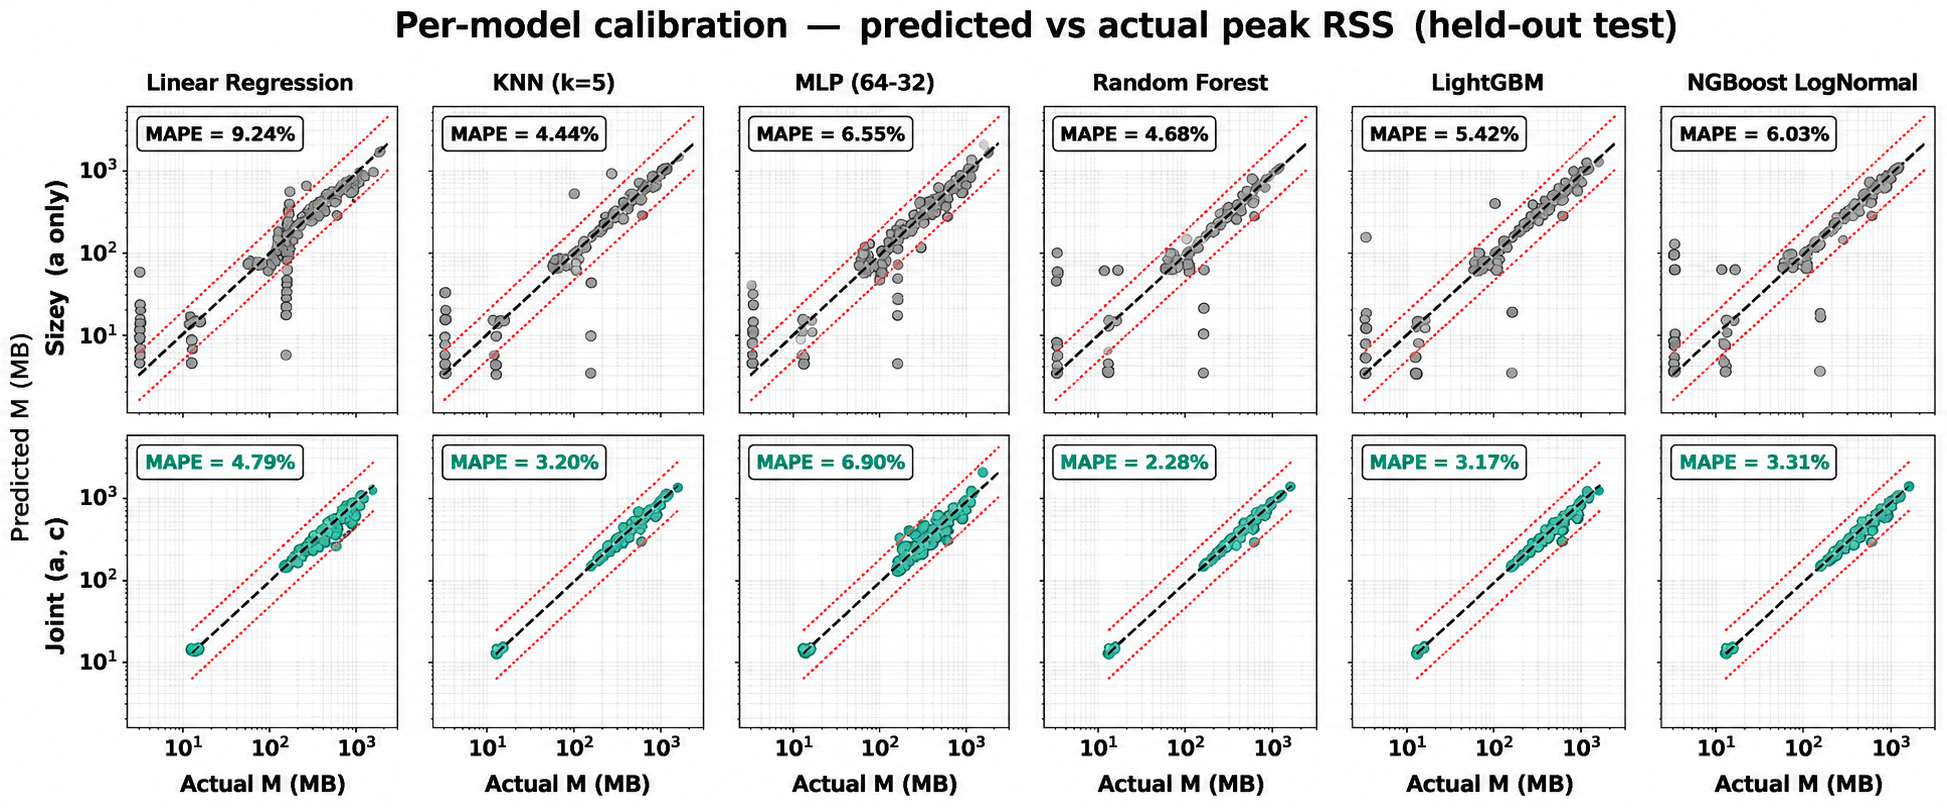
\includegraphics[width=0.9\textwidth,height=0.26\textheight,keepaspectratio]{Figures/Fig_7_Per_model_calibration.png}
\caption{Experiment~1 held-out calibration by model class.
Top row: $\mathbf{x}_{\text{Sizey}} = [\log a(t)]$. Bottom
row: $\mathbf{x}_{\text{Joint}} = [\log a(t), \log c(t)]$.
Black dashed line: perfect calibration; red dotted lines:
factor-of-two envelope. Each panel annotates held-out MAPE.}
\label{fig:exp1:calibration}
\end{figure*}

\paragraph{Comparison against the Sizey ensemble.} The Sizey
ensemble baseline reaches $3.73\%$ MAPE, $0.991$
$R^2_{\log}$, $99.7\%$ Cov.\,$2\times$, $1.819$~GB-hours of
wastage, and $240$ OOMs. LGBM~Joint reduces MAPE to $3.17\%$
and wastage to $0.565$~GB-hours while reducing OOMs to
$221$; RF~Joint reaches $2.28\%$ MAPE and $0.477$~GB-hours
wastage at $245$ OOMs. LGBM~Joint offers the best balance of
accuracy and OOM safety as a replacement for the published
baseline.

\paragraph{Deployment-time memory bookings.}
Held-out MAPE measures predictor accuracy; the cluster-side
quantity is how much memory is actually booked per task at
submission time. Table~\ref{tab:exp1-bookings} reports, for
each Experiment~1 workflow, the median predicted allocation
under the cheap $a$-only feature and under the joint
$\mathbf{x}_{\text{Joint}} = [\log a(t), \log c(t)]$
configuration that follows the \texttt{strace} audit. For six of the seven workflows, the audited median falls to
between $2\%$ and $19\%$ of the cheap median (chipseq from
$1{,}180$~MB to $20$~MB, rnaseq from $881$ to $18$, eager
from $3{,}524$ to $656$). pyradiomics is the exception, with
the median moving from $744$ to $723$~MB -- consistent with
its access pattern where $c(t) \approx a(t)$ and the two
feature views agree.

\begin{table}[t]
\centering
\caption{Experiment~1 deployment-time memory bookings per
workflow. Median predicted allocation (MB) under the cheap
$a$-only feature and under the joint feature view following
\texttt{strace} audit, computed over held-out tasks.}
\label{tab:exp1-bookings}
\footnotesize
\setlength{\tabcolsep}{4pt}
\renewcommand{\arraystretch}{1.15}
\begin{tabular}{|l|c|c|c|}
\hline
\textbf{Workflow} & \textbf{Tasks} & \textbf{Cheap (MB)} & \textbf{Audit (MB)} \\
\hline
chipseq        & 213   & 1{,}180.3 & 20.4   \\ \hline
eager          & 36    & 3{,}524.4 & 655.6  \\ \hline
mag            & 25    & 1{,}202.4 & 66.0   \\ \hline
mag\_karlsson  & 11    & 3{,}524.4 & 655.6  \\ \hline
methylseq      & 36    & 1{,}471.7 & 104.1  \\ \hline
pyradiomics    & 6{,}516 & 744.2   & 722.6  \\ \hline
rnaseq         & 78    & 881.1     & 17.9   \\ \hline
\end{tabular}
\end{table}

\paragraph{Prediction error as a function of task size.}
Figure~\ref{fig:exp1:error-vs-size} sorts held-out rows by
peak RSS into $25$ quantile bins and plots mean APE per bin.
The dominant failure mode of $\mathbf{x}_{\text{Sizey}}$ is
small-task error: in the smallest bin ($\sim 13$~MB), LR
reaches $27.7\%$, LGBM $33.0\%$, RF $45.4\%$, and NGBoost
$61.0\%$. This bin is dominated by
\texttt{pyradiomics::merge\_sample\_features} and
\texttt{iwd::graphToShapefile} -- exactly the small irregular
tasks for which input file size is a weak proxy for memory
demand. Adding $c(t)$ compresses small-task error to
$5$--$8\%$ for all joint models except MLP; RF, LGBM, and
NGBoost stay near or below $5\%$ across the full memory
range.

\begin{figure}[htbp]
\centering
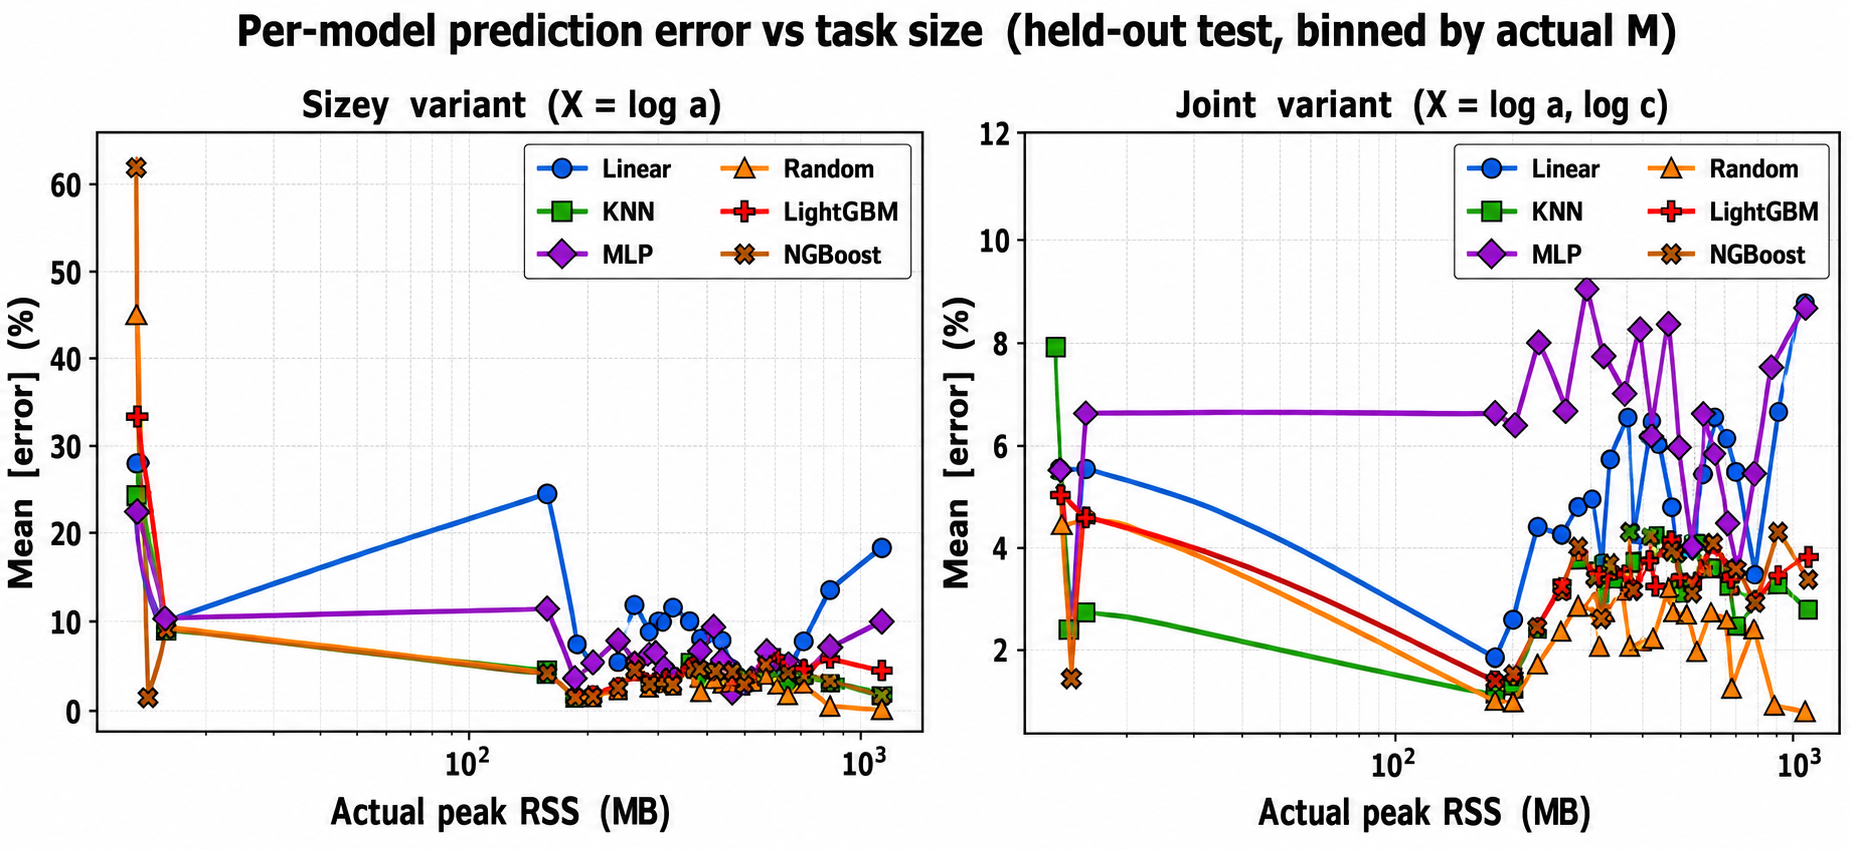
\includegraphics[width=\columnwidth]{Figures/Fig_8_per_model_prediction_error.png}
\caption{Experiment~1 held-out error as a function of task
size. Held-out rows sorted by peak RSS into $25$ quantile
bins; each point is the mean APE in a bin. Left:
$\mathbf{x}_{\text{Sizey}}$. Right:
$\mathbf{x}_{\text{Joint}}$.}
\label{fig:exp1:error-vs-size}
\end{figure}

\subsection{Experiment~2: Prediction Quality Under eBPF Audit}
\label{sec:exp2}

Table~\ref{tab:exp2-final} reports held-out metrics for the
three probabilistic model classes under both feature
configurations and both per-bucket and workflow-global
variants. We use the predictive median as the point estimate
to avoid the instability of the raw LogNormal mean on wide
posteriors.

\begin{table}[t]
\centering
\caption{Experiment~2 held-out results under the eBPF audit.
Boldface marks the best value within each model class for a
given metric.}
\small
\label{tab:exp2-final}
\footnotesize
\setlength{\tabcolsep}{3pt}
\renewcommand{\arraystretch}{1.12}
\begin{tabular}{|l|l|c|c|c|}
\hline
\textbf{Model} & \textbf{Variant} & \textbf{MAPE} & \textbf{$R^2_{\log}$} & \textbf{Cov.\,2$\times$} \\
\hline
\multirow{4}{*}{NGBoost}
  & Sizey               & 30.77            & 0.966            & \textbf{93.1} \\
\cline{2-5}
  & Joint               & 22.43            & 0.970            & 91.4 \\
\cline{2-5}
  & Glob.\ Sizey        & 32.42            & 0.964            & 89.3 \\
\cline{2-5}
  & Glob.\ Joint        & \textbf{19.30}   & \textbf{0.972}   & 90.4 \\
\hline
\multirow{4}{*}{Q-LGBM}
  & Sizey               & \textbf{16.12}   & 0.944            & 92.1 \\
\cline{2-5}
  & Joint               & 17.60            & \textbf{0.956}   & \textbf{93.4} \\
\cline{2-5}
  & Glob.\ Sizey        & 42.27            & 0.927            & 91.4 \\
\cline{2-5}
  & Glob.\ Joint        & 20.58            & \textbf{0.956}   & 93.2 \\
\hline
\multirow{4}{*}{BayesRidge}
  & Sizey               & 22.68            & 0.969            & 89.7 \\
\cline{2-5}
  & Joint               & \textbf{22.52}   & \textbf{0.970}   & \textbf{90.4} \\
\cline{2-5}
  & Glob.\ Sizey        & 103.61           & 0.843            & 60.9 \\
\cline{2-5}
  & Glob.\ Joint        & 97.68            & 0.847            & 68.1 \\
\hline
\end{tabular}
\end{table}

Adding $c(t)$ improves every NGBoost metric and both Bayesian
Ridge metrics; Quantile LightGBM trades a small MAPE increase
for better coverage. The architectural question is whether
the per-bucket structure of \S\ref{sec:model-granularity}
remains necessary once the predictor consumes both $a(t)$ and
$c(t)$. The answer is model-dependent: NGBoost~Joint is the
only case where the global variant beats its per-bucket
counterpart on MAPE ($19.30$ vs.\ $22.43$). Q-LGBM and
Bayesian Ridge global variants degrade substantially -- the
global Bayesian Ridge fails to fit cross-bucket structure
entirely.

\begin{figure}[t]
\centering
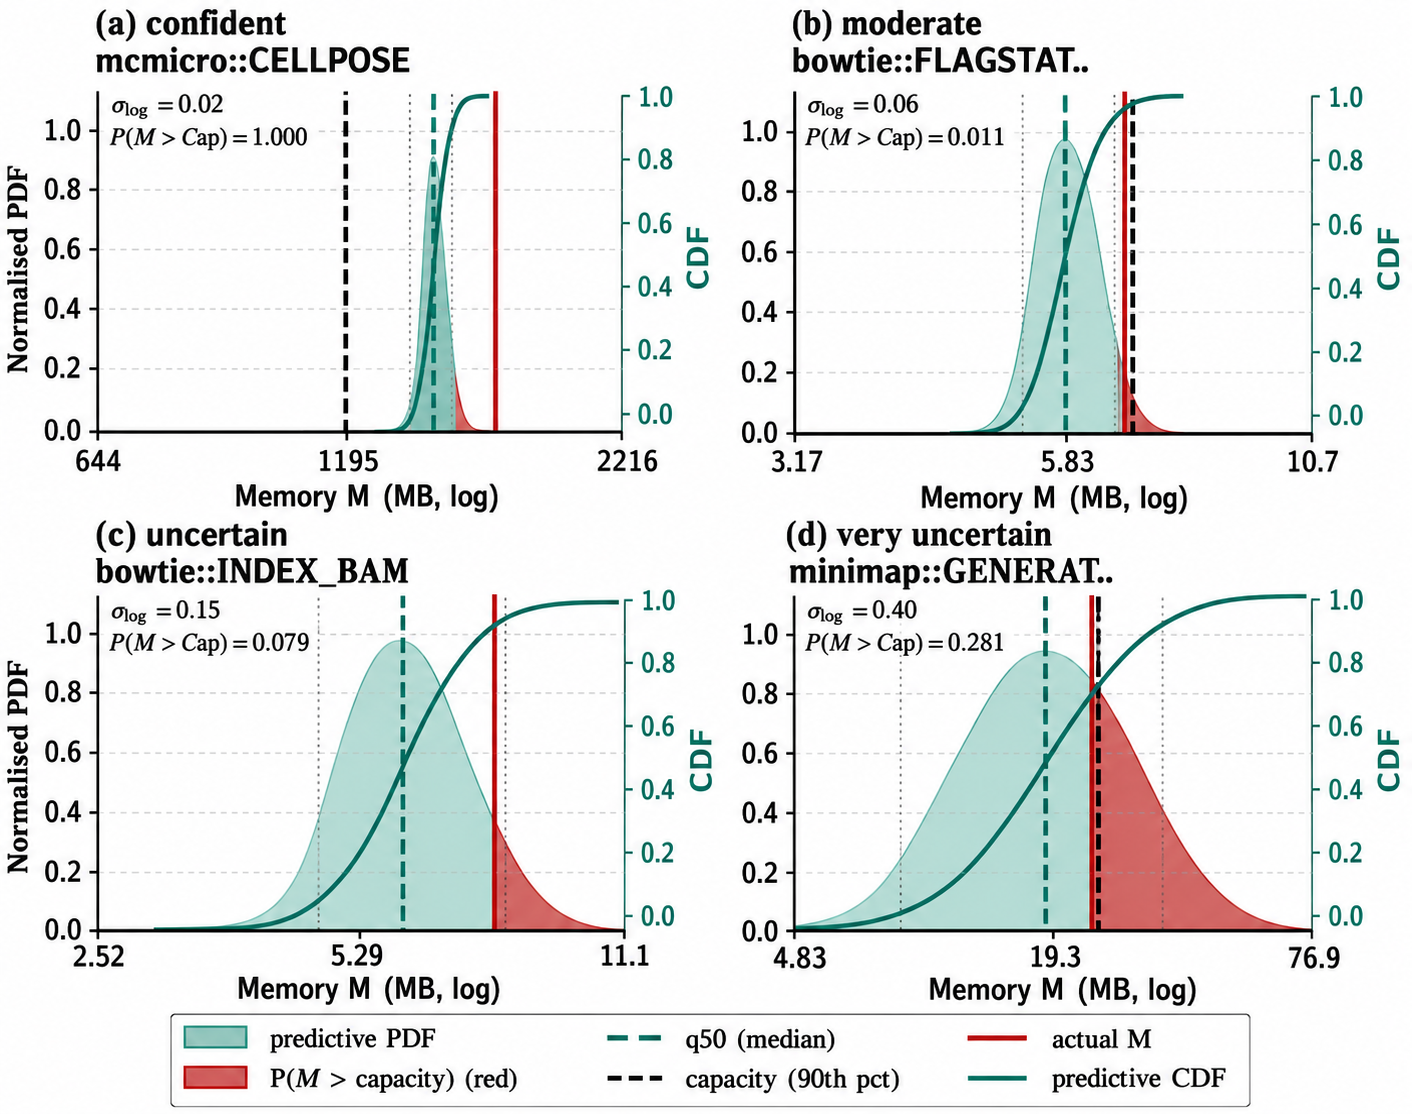
\includegraphics[width=\columnwidth]{Figures/Fig_9_Enhanced.png}
\caption{Experiment~2 representative NGBoost~Joint predictive
distributions on held-out tasks across confident, moderate,
uncertain, and very uncertain regimes. Filled green:
predictive PDF; green line: predictive CDF; red line:
realised peak memory; black dashed line: bucket capacity
($90$th-percentile of training memory). Red shaded tail is
$P(m(t) > \text{cap}(t))$, the score consumed by the
active-learning gate of Experiment~3.}
\label{fig:e2:cdf}
\end{figure}

Figure~\ref{fig:e2:cdf} makes the gate input concrete: in
confident panels the predictive distribution sits below
capacity and the tail mass above is negligible; as
uncertainty grows the right tail overlaps capacity, raising
$P(m(t) > \text{cap}(t))$. This is the quantity the
deployment gate uses to route incoming tasks through the
eBPF audit lane.

\subsection{Experiment~3: Active-Learning Convergence}
\label{sec:exp3}

Experiments~1 and~2 assume every audited tuple is available at
training time. Experiment~3 drops that assumption: the
predictor starts from a small uniform seed and grows its
labelled pool round by round under the gate of
\S\ref{sec:solution}, with audit decisions driven by the
current predictor's posterior. We instantiate the protocol
twice in parallel -- once on the Experiment~1 setting (point
predictor, offline \texttt{strace}) and once on the
Experiment~2 setting (distribution predictor, online eBPF).

\paragraph{Protocol.} Round~$0$ exposes $c(t)$ for a
uniformly-sampled $5\%$ of training rows and fits the joint
$(a, c)$ predictor on that seed. Each subsequent round scores
non-audited rows using the active-learning composite of
\S\ref{sec:solution}, audits the top-$5\%$, and refits on the
cumulative audited pool under importance weights
$1/p_t$~\cite{horvitz1952generalization}, where $p_t$ is the
row's cumulative selection probability. Five rounds end at
$30\%$ cumulative audit. The random baseline uses the same
schedule with uniform draws; the oracle is the joint
predictor trained on the full $80\%$ partition. The point
predictor reads $G_1$ off the NGBoost LogNormal
$\sigma_{\log}$, $G_2$ off $P(m(t) > \text{cap}(t))$
computed from the same NGBoost head, and $G_3$ off inverse
bucket count. The distribution predictor reads $G_1$ off the
Q-LGBM log-space quantile spread, $G_2$ off the same
$P(m(t) > \text{cap}(t))$ from the quantile triplet, and
$G_3$ from the same inverse bucket count.

\paragraph{Results.}
Figure~\ref{fig:e3:al-curves} reports held-out MAPE and
wastage as the cumulative audit fraction grows from $0.05$ to
$0.30$. Across both predictor types, the gate-driven loop
tracks random sampling within the noise band of the held-out
partition rather than dominating it. With the point
predictor, gate MAPE oscillates between $2.99\%$ (seed) and
$3.59\%$ at $30\%$ audit while random reaches $3.11\%$, and
gate wastage rises from $188$~MB at the seed to $308$~MB at
$30\%$ audit while random stays near $200$--$330$~MB across
the same budgets; OOM counts move $327 \to 302$ for gate
vs.\ $330 \to 281$ for random. With the distribution
predictor, random reaches $2.67\%$ MAPE at $30\%$ audit while
the gate oscillates in the $3$--$4\%$ range, and random
delivers lower OOM counts at four of five budgets. The
full-audit oracle is $3.01\%$ MAPE for the point setting and
$2.32\%$ for the distribution setting.

\begin{figure}[t]
\centering
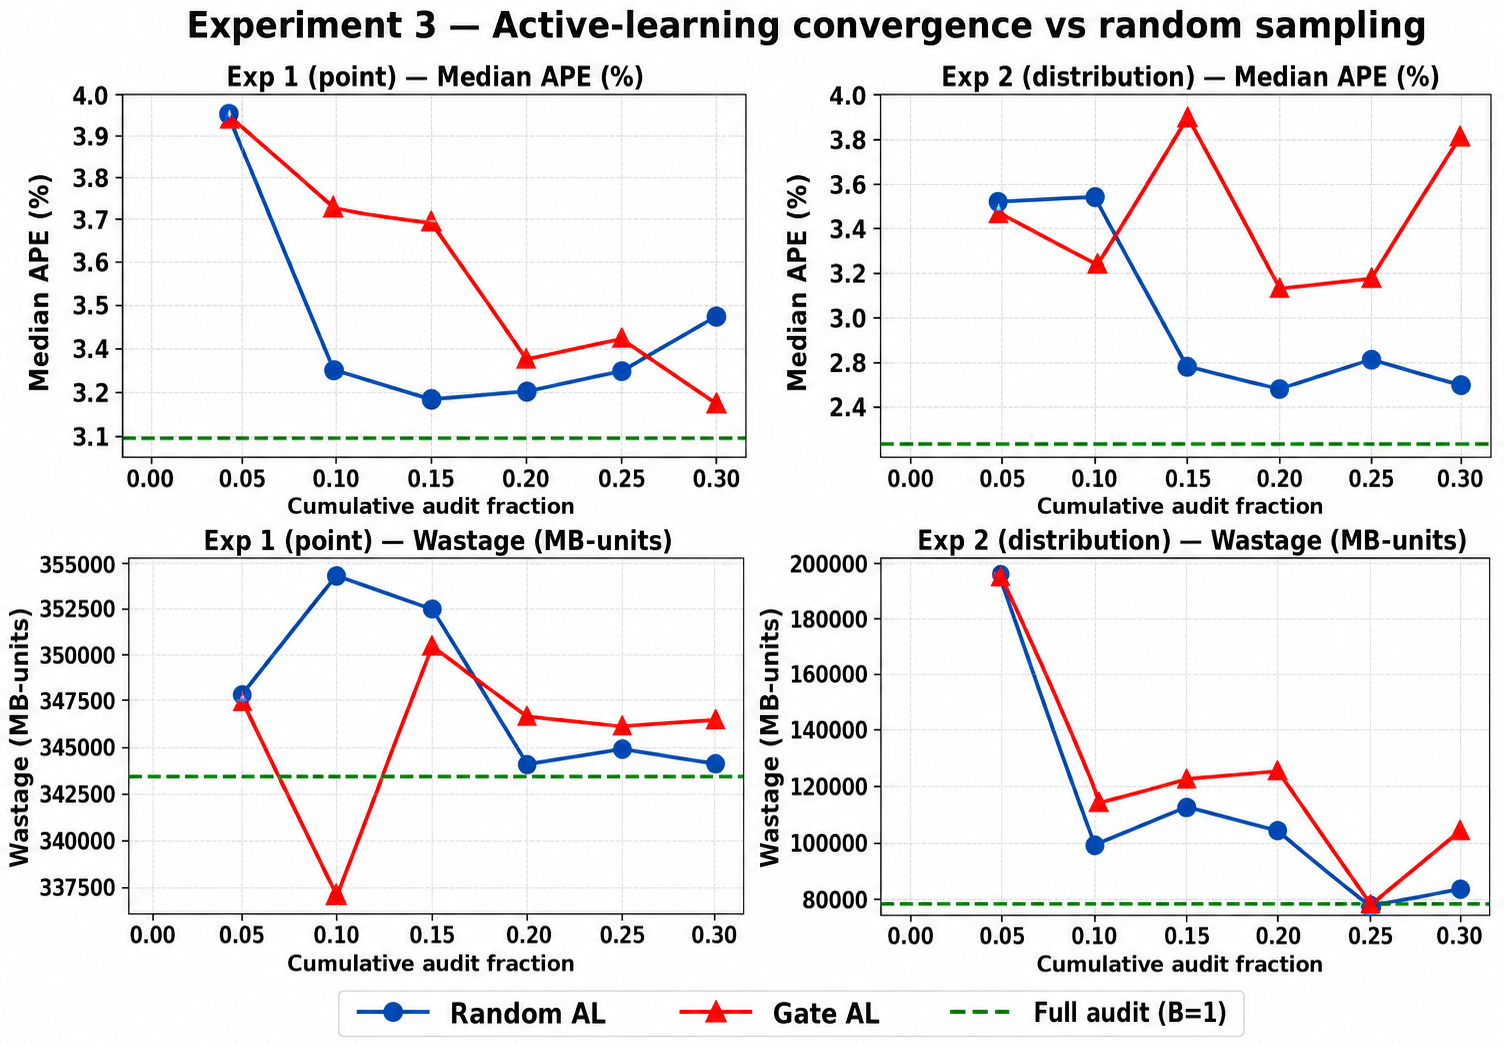
\includegraphics[width=\columnwidth]{Figures/Fig_10_Exp_3.png}
\caption{Experiment~3 active-learning convergence. Top row:
held-out MAPE vs.\ cumulative audit fraction. Bottom row:
held-out wastage. Left column: point predictor (NGBoost
gate). Right column: distribution predictor (Q-LGBM gate).
Dashed line: full-audit oracle ($B = 1$). The gate-driven
loop tracks random sampling within noise across both
regimes.}
\label{fig:e3:al-curves}
\end{figure}

\paragraph{Why informed sampling does not improve over random.}
Both gate signals are dominated by training-set sparsity
rather than prediction error: with buckets of $10$--$40$
instances, $\sigma_{\log}$ is largely fold-variation noise, so
the gate biases the audited pool toward rare buckets and IPW
amplifies the bias. The full-audit oracle ($3.01\%$ MAPE) is
itself barely better than random at $10\%$ budget ($2.76\%$),
leaving informed sampling no slack to exploit.

\subsection{Discussion}
\label{sec:discussion}

% The three campaigns yield three transferable findings.
% First, $c(t)$ is a complementary feature to $a(t)$ rather
% than a replacement: every model class in Experiment~1 either
% improves on its $a$-only counterpart (five of six) or fails
% to exploit it cleanly (MLP). The improvement is largest for
% boosted ensembles and Random Forest -- the models most
% sensitive to small-task heterogeneity in the input-size
% feature.

% Second, the per-bucket structure carried over from Sizey
% remains useful in the joint configuration but its necessity
% is predictor-dependent: per-bucket variants dominate the
% global fallback for point regressors and Q-LGBM, only
% NGBoost~Joint absorbs enough between-bucket variation that
% the global variant becomes competitive on MAPE, and Bayesian
% Ridge global degrades catastrophically -- consistent with
% linear-Gaussian regression failing on a heavy-tailed
% cross-bucket distribution.

% Third, the active-learning gate's value at our scale is
% architectural rather than statistical (\S\ref{sec:exp3}):
% the same predictor produces both the safe allocation and
% the audit signals, with no separate model to maintain, even
% though gate-driven sampling does not improve over uniform
% sampling at the bucket sparsity present in our workloads.

The experimental results yield three transferable findings, one qualification, and one open question.
First, data consumption $c(t)$ improved five of six models, with the sharpest gains in the sub-50 MB regime where aggregate I/O ($a(t)$) is least informative. In workflows like chipseqand rnaseq, audited median allocations dropped to ~2\% of "cheap" estimates. Conversely, for tasks where $c(t) \approx a(t)$, such as pyradiomics, the gate correctly identified the audit as low-value. Given the high cost of OOMs, LGBM Joint is the recommended default, providing the best balance of accuracy ($3.17\%$ MAPE) and minimal wastage.

Second, per-bucket structures are necessary for most predictors. Per-bucket variants generally outperform global models. The exception is NGBoost Joint, where a global model achieved lower MAPE ($19.30\%$) than its per-bucket counterpart. This suggests that with both $a(t)$ and $c(t)$ available, NGBoost’s distributional head absorbs enough variation to make task-type boundaries redundant.

Third, MAPE variance reflects dataset difficulty. Higher MAPE in Experiment 2 (16–30\%) compared to Experiment 1 (2–6\%) stems from workload complexity, not model failure. The eBPF workloads span wider memory ranges with lower per-bucket instance counts. While models converge easily on large datasets (e.g., 3,500+ instances in pyradiomics), the Experiment 2 results better characterize "hard" prediction settings with high heterogeneity.

Finally, we see that active-learning gates match random sampling at small scales. At our current scale, gate-driven sampling performed similarly to random sampling. With small bucket populations (10–40 instances), uncertainty signals are often dominated by training-fold noise. While the gate concentrates audits on rare buckets, random sampling better preserves the population distribution for generalization. %The gate's current value is architectural—using one model for both allocation and auditing signals—rather than statistical. 
This leads to open question about statistical utility. We believe that the transition from architectural to statistical utility likely depends on bucket population size and workload heterogeneity. We estimate a threshold of 200–300 instances per bucket for informed sampling to consistently outperform random selection. %Future large-scale deployments are required to determine how optimal gating weights $(w_U, w_R, w_N)$ vary across different workload families.